\documentclass[12pt]{article}
\usepackage{amssymb,amsfonts,amsmath}
\usepackage{tikz}
\usepackage{pgfplots}
\usetikzlibrary{shapes}
\newcommand{\picdir}{pdffig}

\usepackage[top=0.5in,bottom=0.5in,left=0.5in,right=0.5in]{geometry} % Reduce the size of the margin



\begin{document}
%\tdplotsetmaincoords{60}{120}
\section{FPFDM}

\begin{verbatim}
Semmineh, Natenael B., et al. "An efficient computational approach to
characterize DSC-MRI signals arising from three-dimensional heterogeneous tissue
structures." PloS one 9.1 (2014): e84764.
\end{verbatim}

Field pertubation given by the integral/superposition of finite perturbers over
the field of view
\[
\Delta B =  \int V \Delta B_\text{cube}  = \mathcal{F}^{-1} \left( \mathcal{F} V(C_T) \mathcal{F} \Delta B_\text{cube} \right)
\]
Where
\[
\Delta B_\text{cube}  = \frac{ 6 \Delta \chi R^3} {\pi 3 r^3} (3 \cos^2 \theta-1) B_0
\]
Here, $V$ includes the  structure information as well as concentration $C_T$
information from flow simulation to
where the Gadolemium concentration is within the structure, $V(C_T)$.

Time explicit finite difference on Bloch equations to solve for magnetization
\[
M(t+\Delta t) = \Phi(t) \otimes (I+A)M(t)
\]
Field pertubations appear in RHS of Bloch solve
\[
\Phi(t) = [ \dots \exp(-i \gamma \Delta B_k \Delta t - \Delta t / T2_k) \dots ] 
\]
MR signal is sum over the FOV
\[
S(t) = \frac{1}{M_0} \sum_k M_k(t)
\]
Transverse relaxation rates are calculated at the echo time and are proportional
to the concentration curves from Rohan, $C_T(t)$
\[
\Delta R_2 = - \frac{ ln S(TE)}{TE} = k \cdot C_T(t)
\]
{\color{red} Possible circular arguement here. $C_T$ was already used to get the
Feild perturbation. Need to look up derivation of $\Delta R_2$, MTT etc to
determine what is appropriate for the final comparison.}

Tissue blood flow, tissue blood volume and MTT are obtained from the
concentration, $C_T(t)$ and AIF, $C_A$.
\[
C_T(t) = TBF \int_0^t C_A(\tau) R (t-\tau) d\tau
\]
\[
TBV = \frac{ \int C_T dt}{\int C_A dt}
\]
\[
MTT = \frac{TBV}{TBF}
\]


\pagebreak
\section{Derivations}
Adapting  the interpretation of 

\begin{verbatim}
Meier, P., & Zierler, K. L. (1954). On the theory of the indicator-dilution
method for measurement of blood flow and volume. Journal of applied physiology,
6(12), 731-744.

Indicator Dilution Methods for Measuring Blood Flow, Volume,
and Other Properties of Biological Systems:
A Brief History and Memoir
KENNETH ZIERLER
\end{verbatim}

\begin{figure}[h]
\centering
\scalebox{0.47}{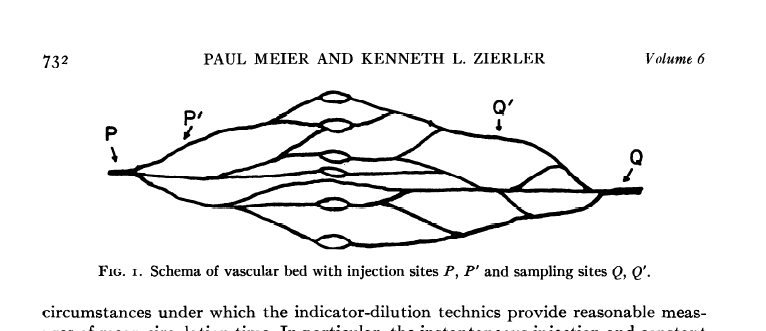
\includegraphics{\picdir/dscintuition.png}}
\caption{Representative blood flow
} \label{fig:DSCbloodflow}
\end{figure}

The whole point of DSC indicator dilution theory is to ignore the complex
vasculature. Consider an incompressible fluid flowing through the vasculature in Figure~\ref{fig:DSCbloodflow}.
Consider a mass injection $q [kg]$ within a flowing fluid at point $P$ 
We \textbf{assume} the fluid is flowing with a mass flow $F[m^3/s]$. 
The mass injection is diluted within the flowing fluid and appears as a
concentration, $c[kg/m^3]$,  at point $Q$.
Mass balance the total exiting equal the input
\[
    q [kg] = \int_0^\infty c[kg/m^3]F[m^3/s] \;dt  \qquad \Rightarrow  \qquad F = \frac{q }{\int_0^\infty c}
\]
We define the fraction exiting the system per time as $h$.
\[
      h(t)[1/s] = \frac{F [m^3/s] c [kg/m^3]}{q[kg]} \qquad \Rightarrow \qquad \int_0^\infty h(t) dt = 1
\]

The volume of fluid entering the system over time $t$ is the flow rate times
time for the incompressible fluid in the static vessel structure.
\[
  F[m^3/s] t = \text{volume entering or exiting \color{red} unclear why we use t here and not dt ? }
\]
We  will \textbf{assume} $h \; dt$ is the volume fraction exiting the system.
Implicitly, we are assuming the that density of the indicatory within the
flowing fluid remains at the same density. 
Thus the volume of indicator exiting the system is the volume of the fluid times
the volume fraction of the indicator
\[
   V = \int_0^\infty t [s] F[m^3/s] h(t) [1/s] dt [s]
\qquad \Rightarrow \qquad
   \frac{V}{F} = \int_0^\infty t  h(t)  dt  = \text{MTT}
\]
Either way, need to reduce full scale 1d model from rohan down to these
assumptions. Within a voxel we need to accumulate one entry 'P' and one exit 'Q'
to match full scale to DSC MTT.

\pagebreak
Consider mass flow, $F[m^3/s]$ through a cylindrical vessel over time $\Delta t [s]$.
For a given concentration, $c[kg/m^3]$, we will define $h(t) [1/s] \Delta t [s]$
as the (mass or volume? ) fraction of the original mass injection, $q_i [kg]$
\[
    q_i [kg] h(t) [1/s] \Delta t [s] \equiv F[m^3/s] c[kg/m^3] \Delta t [s]
    = \text{mass in units of kg flowing out of cylinder}
\]
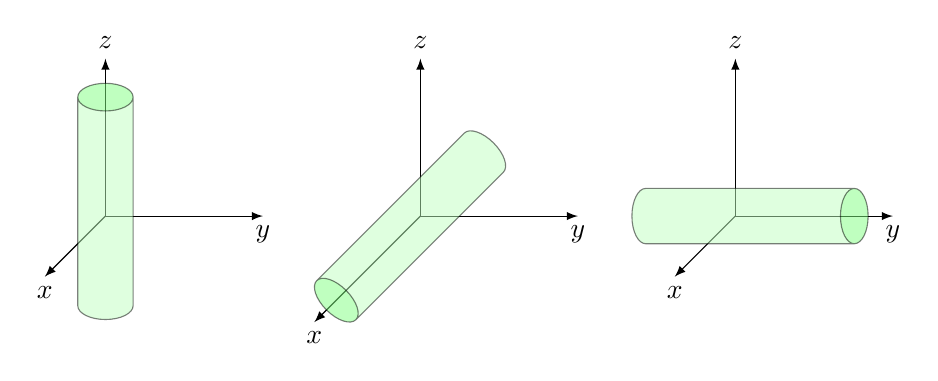
\begin{tikzpicture}

  \coordinate (O) at (0,0,0);
  \coordinate (A) at (2,0,0);
  \coordinate (B) at (0,2,0);
  \coordinate (C) at (0,0,2);

        % draw axis
  \draw[-latex] (O) -- (A) node[below] {$y$};
  \draw[-latex] (O) -- (B) node[above] {$z$};
  \draw[-latex] (O) -- (C) node[below] {$x$};

    \node[cylinder, draw, shape aspect=.5, 
      cylinder uses custom fill, cylinder end fill=green!50, 
      minimum height=1cm,
      cylinder body fill=green!25, opacity=0.5, 
    scale=3, rotate=90]{};

  \begin{scope}[shift={(4,0)}]

    \coordinate (O) at (0,0,0);
    \coordinate (A) at (2,0,0);
    \coordinate (B) at (0,2,0);
    \coordinate (C) at (0,0,3.5);

        % draw axis
    \draw[-latex] (O) -- (A) node[below] {$y$};
    \draw[-latex] (O) -- (B) node[above] {$z$};
    \draw[-latex] (O) -- (C) node[below] {$x$};

    \node[cylinder, draw, shape aspect=.5, 
      cylinder uses custom fill, cylinder end fill=green!50, 
      minimum height=1cm,
      cylinder body fill=green!25, opacity=0.5, 
    scale=3, rotate=-135]{};
  \end{scope}
  \begin{scope}[shift={(8.,0)}]

    \coordinate (O) at (0,0,0);
    \coordinate (A) at (2,0,0);
    \coordinate (B) at (0,2,0);
    \coordinate (C) at (0,0,2);

        % draw axis
    \draw[-latex] (O) -- (A) node[below] {$y$};
    \draw[-latex] (O) -- (B) node[above] {$z$};
    \draw[-latex] (O) -- (C) node[below] {$x$};


    \node[cylinder, draw, shape aspect=.5,  
      cylinder uses custom fill, cylinder end fill=green!50, 
      minimum height=1cm,
      cylinder body fill=green!25, opacity=0.5, 
    scale=3]{};


  \end{scope}


\end{tikzpicture}

With this definition of $h[1/s]$, we can interpret
\[
 F [m^3/s] h(t) [1/s] \Delta t [s] 
\]
as the fraction of  the total flow, $F$ that exists. 
From the geometrical relation, the volume occupied is the length of the cylinder
at time $t$ times the area within the time $t+ \Delta t$.
\[
 \text{distance} =  c [m/s] \cdot t [s]
\qquad
 \text{area} =  \frac{F [m^3/s]}{c[m/s]} 
\]
THus the volume traversed by the mass fraction is the 
\[
 \text{distance * area * mass fraction} =  c [m/s] \cdot t [s]
 \cdot \frac{F [m^3/s]}{c[m/s]}   h(t) [1/s] \Delta t [s] 
  = t F h(t) dt
\]

\end{document}
